\chapter{Concept Design and Implementation}
\section{Research Direction}
As mentioned earlier, the scope of the design discussed in this paper has gradually narrowed from a broad scope, but the direction of research and the main key ideas have not changed much, namely how to make users feel their own or the motion trajectory and motion state of the role they manipulate. How can users realize that when they perform a certain action in the virtual space, they are indeed actively doing a certain action spontaneously, rather than just moving their hands or controllers to a specified location according to the guidance of the system. A more abstract explanation is, how can users feel the quality and realism of the action. Can we use some kinematic or haptic devices to convey the action quality of the objects they manipulate in the virtual space to the users, or sufficiently specific action information, to assist users in subjectively or objectively adjusting the amplitude and intensity of their own actions.

Instead of interacting with static objects or those set into motion by external forces, such as a ball being hit, the difference from previous studies is that the target object manipulated by the user in this study has a certain autonomous ability. These are not mere reactive moving state, but self-moving state.

Alternatively referred to as a haptic display device of motion state information for self-moving objects, this technology can be implemented in a wide array of automation systems. These can range from vehicles and drones to robots, or even avatars in virtual environments, thereby opening up extensive applications.

\section{Prototype Version 1 -Katana}
\subsection{Concept Design}
In the initial design attempt, it started with the most common handheld weapon in the virtual environment as a reference and acting object. 

The design goal is to develop a system that can simulate the motion state of the user's handheld object in a virtual environment, such as a weapon. The initial implementation scenario also started with the basic parry action in fencing as the output target. 

This parry mechanism is widely used in action game design, so in the early ideal application scenario, we hope to be able to effectively show high-quality parrying actions of swordsmen through haptic. After the user swings out the controller used as a weapon and successfully parries, the kinematic feedback caused by the recoil force of the parry will be generated so that the user can show the same parrying action interaction as shown in the real swordsman duel.

\begin{figure}[h]
\centering
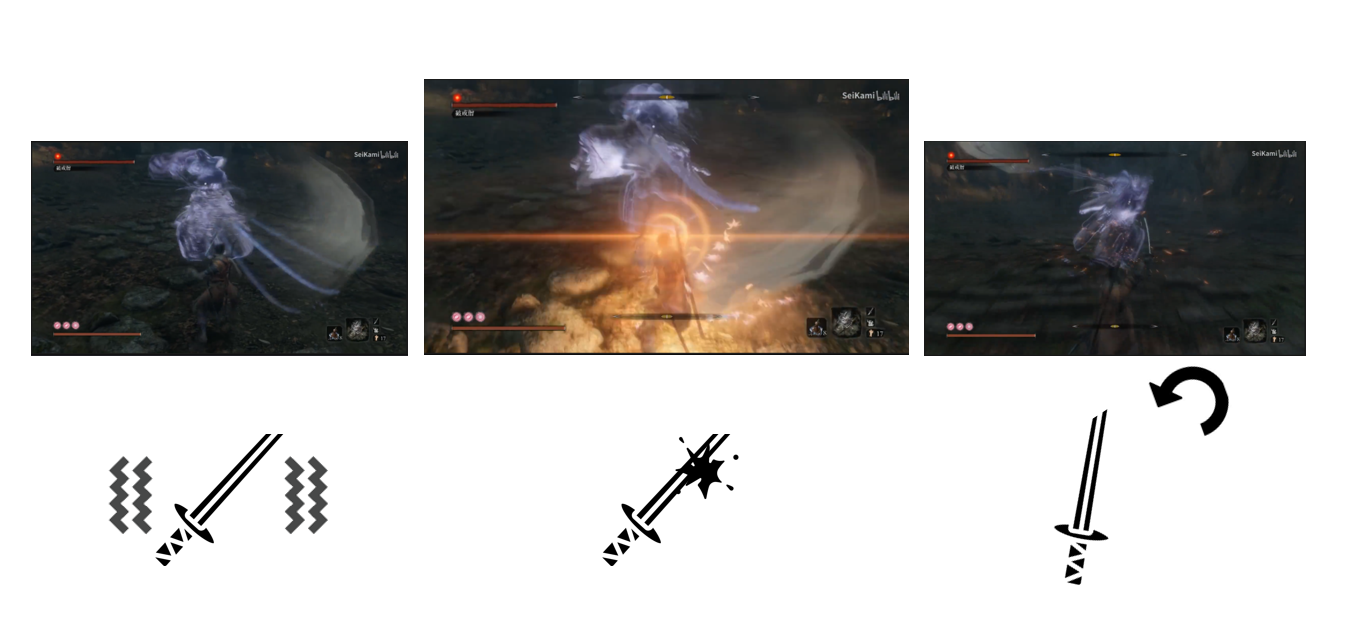
\includegraphics[width=0.6\textwidth]{A_thesis/figures/032.png}
\caption{Ideal scenario}
\end{figure}

In the prototype design, a solenoid is also used as the main source of mechanical output, because the design goal is to simulate the recoil force similar to the impact force. The common driven physical force representation devices in the force output performance can roughly be divided into three types: solenoids, electronic vibrators, and servo motors. The performance characteristics of each type in mechanics are summarized as follows:

Solenoids: Solenoids are electromagnetic devices that generate haptic feedback by generating a magnetic field in a coil by passing current. When current passes through the coil, the magnetic field generates a force acting on the movable chip. Solenoids usually have a larger force output capacity and higher rigidity. Solenoids are frequently used in locking mechanisms including door locking, car parks and access barriers and they are often used in applications that require higher strength and larger displacement ranges, especially as the impact generator.

Vibrators: Electronic vibrators are haptic device that can generate vibrations. It usually consists of a small motor and eccentric mass (such as eccentric rotary mass or eccentric linear mass). When the motor starts, the eccentric mass will cause the device to vibrate, thereby generating haptic feedback. Vibrators usually have smaller force output and lower stiffness, suitable for applications that require rapid haptic stimulation, such as game controllers and haptic notification devices.

Servo Motors: A servo motor is a haptic device that can provide precise force control and position control. It consists of a motor, sensors, and a feedback control system. The servo motor adjusts the output force according to the position information fed back by the sensor to achieve precise force control. Servo motors usually have higher force output and higher control precision, suitable for applications that require precise force control and position feedback, such as surgical simulators and industrial robots.

The prototype design is to set multiple solenoids on one side of the blade of the sword body, use the solenoids to hit the sword body, simulate the impact force generated by the parry in the virtual environment, and force the user to generate a kinematic response.

\begin{figure}[h]
\centering
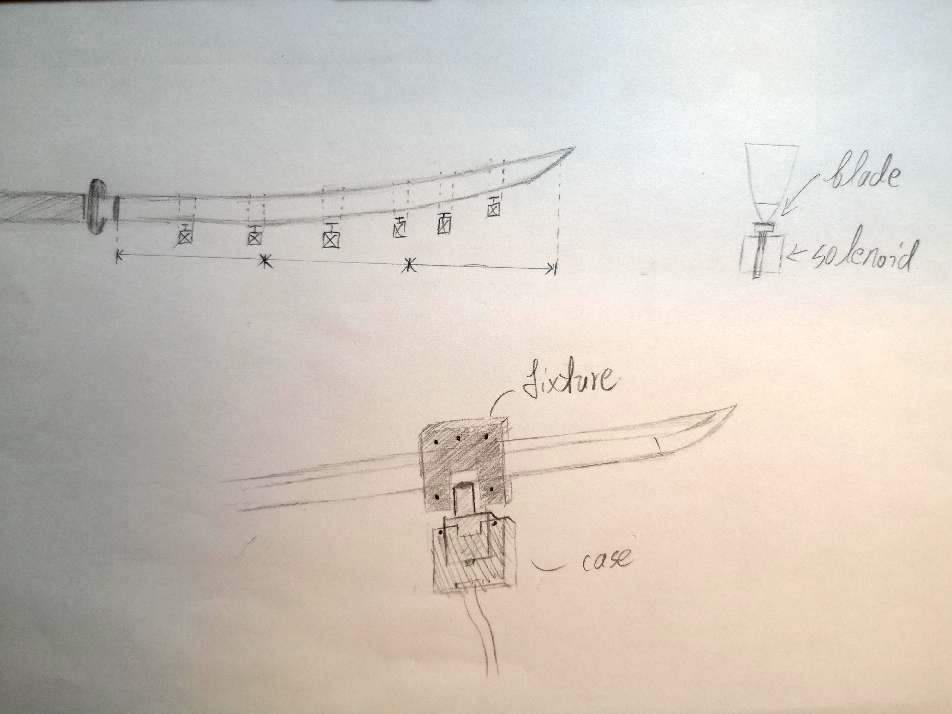
\includegraphics[width=0.6\textwidth]{A_thesis/figures/019.png}
\caption{Early design drafts}
\end{figure}

\subsection{Implement}
\subsubsection{Multi-point Output Control Experimental Circuit}
Considering the principle of voltage shunting, the first attempt is to check whether the 6v circuit on the conventional development board can ensure the output of multiple small 5V solenoids to achieve the purpose of multi-point output.

\begin{figure}[h]
\centering
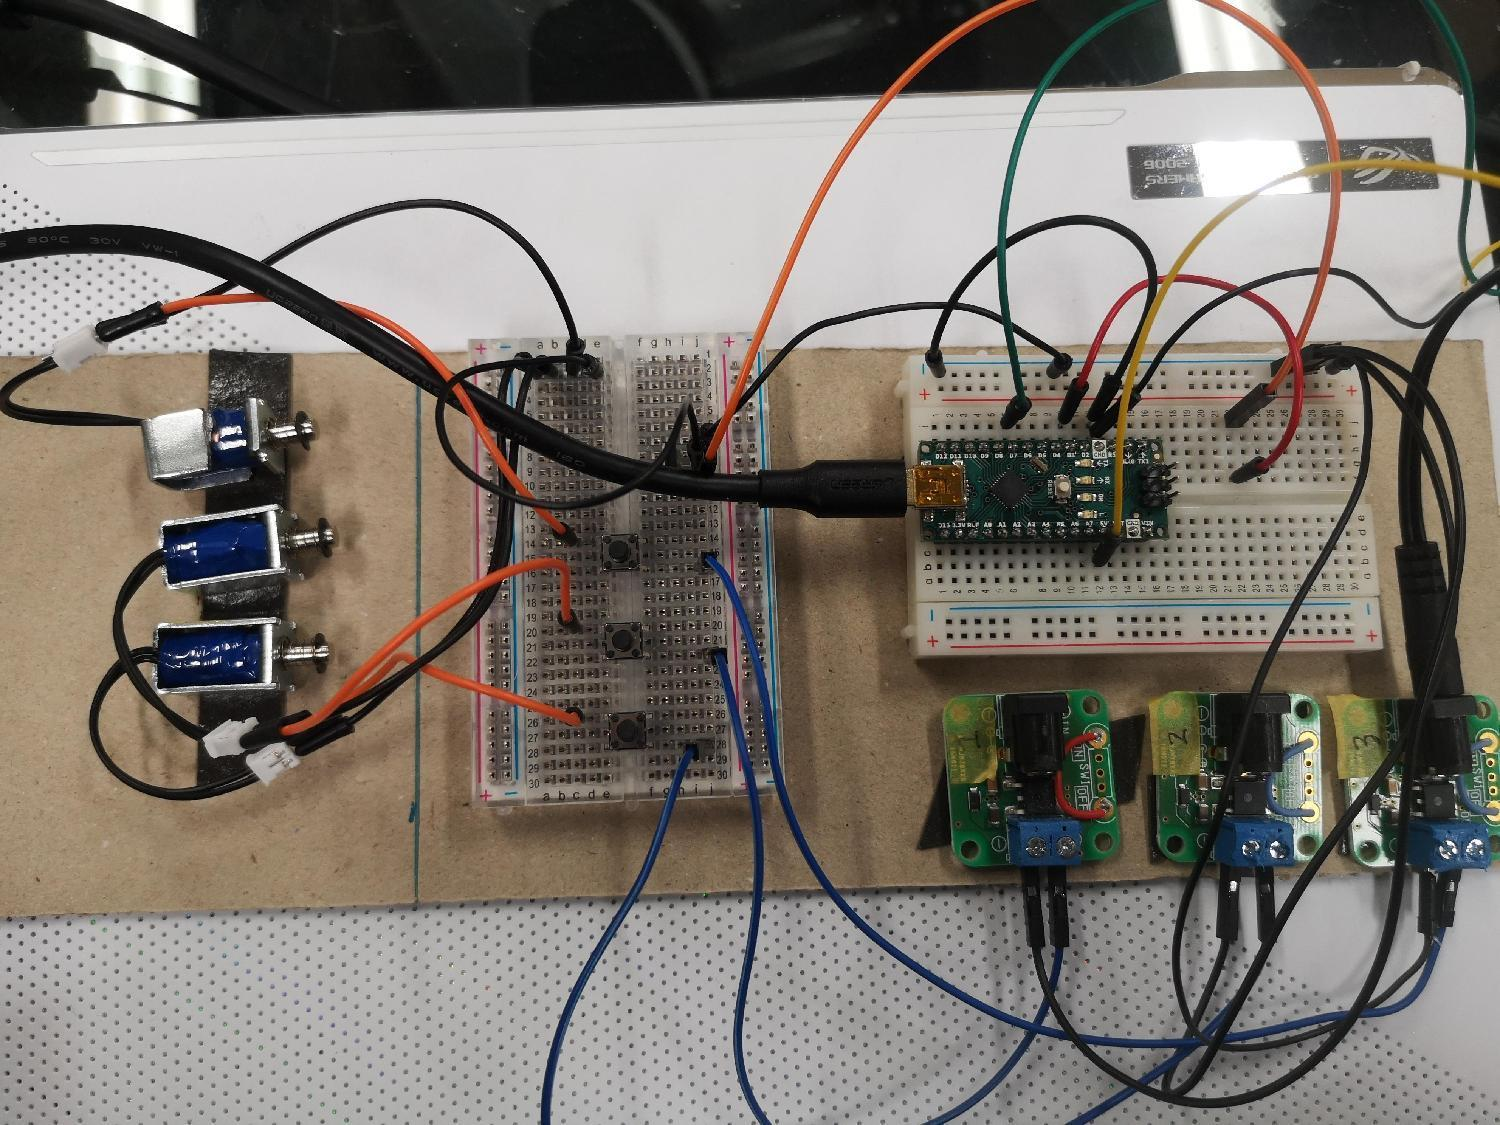
\includegraphics[width=0.6\textwidth]{A_thesis/figures/020.png}
\caption{Experimental Circuit}
\end{figure}

The principle of voltage division, in its practical implementation, has been observed to significantly reduce the standalone power of each component. Therefore, in forthcoming attempts, the primary objective will be the design and implementation of single-point collision detection. This serves as a phased goal, paving the way for further developments.

\subsubsection{Implement Logic Circuit}
The same as the experimental circuit, the initial prototype design also uses the Arduino development board as the main control circuit. At the same time, because we hope that the solenoid device can produce enough kinematic effects, after trying three large-scale, high-output solenoids(12v 1.5A, 24v 0.4A, 24V 1.5A), we chose to use a 24v 1.5A solenoid as the output driver, and used a relay to physically achieve small circuit control of the large circuit, ensuring safety in a high-voltage environment.

\subsubsection{3D Design}
In addition to the core construction, the overall design uses laser printing and 3D printing. To ensure the consistency of the contact points of the solenoids and the blade, laser cutting is used to make the fixtures for the blades.
The solenoids are carried in a 3D printed box under the fixture. At the link point, because no suitable materials were found at the time, only a wooden stick was used as the connector between the two parts.

\begin{figure}[h]
\centering
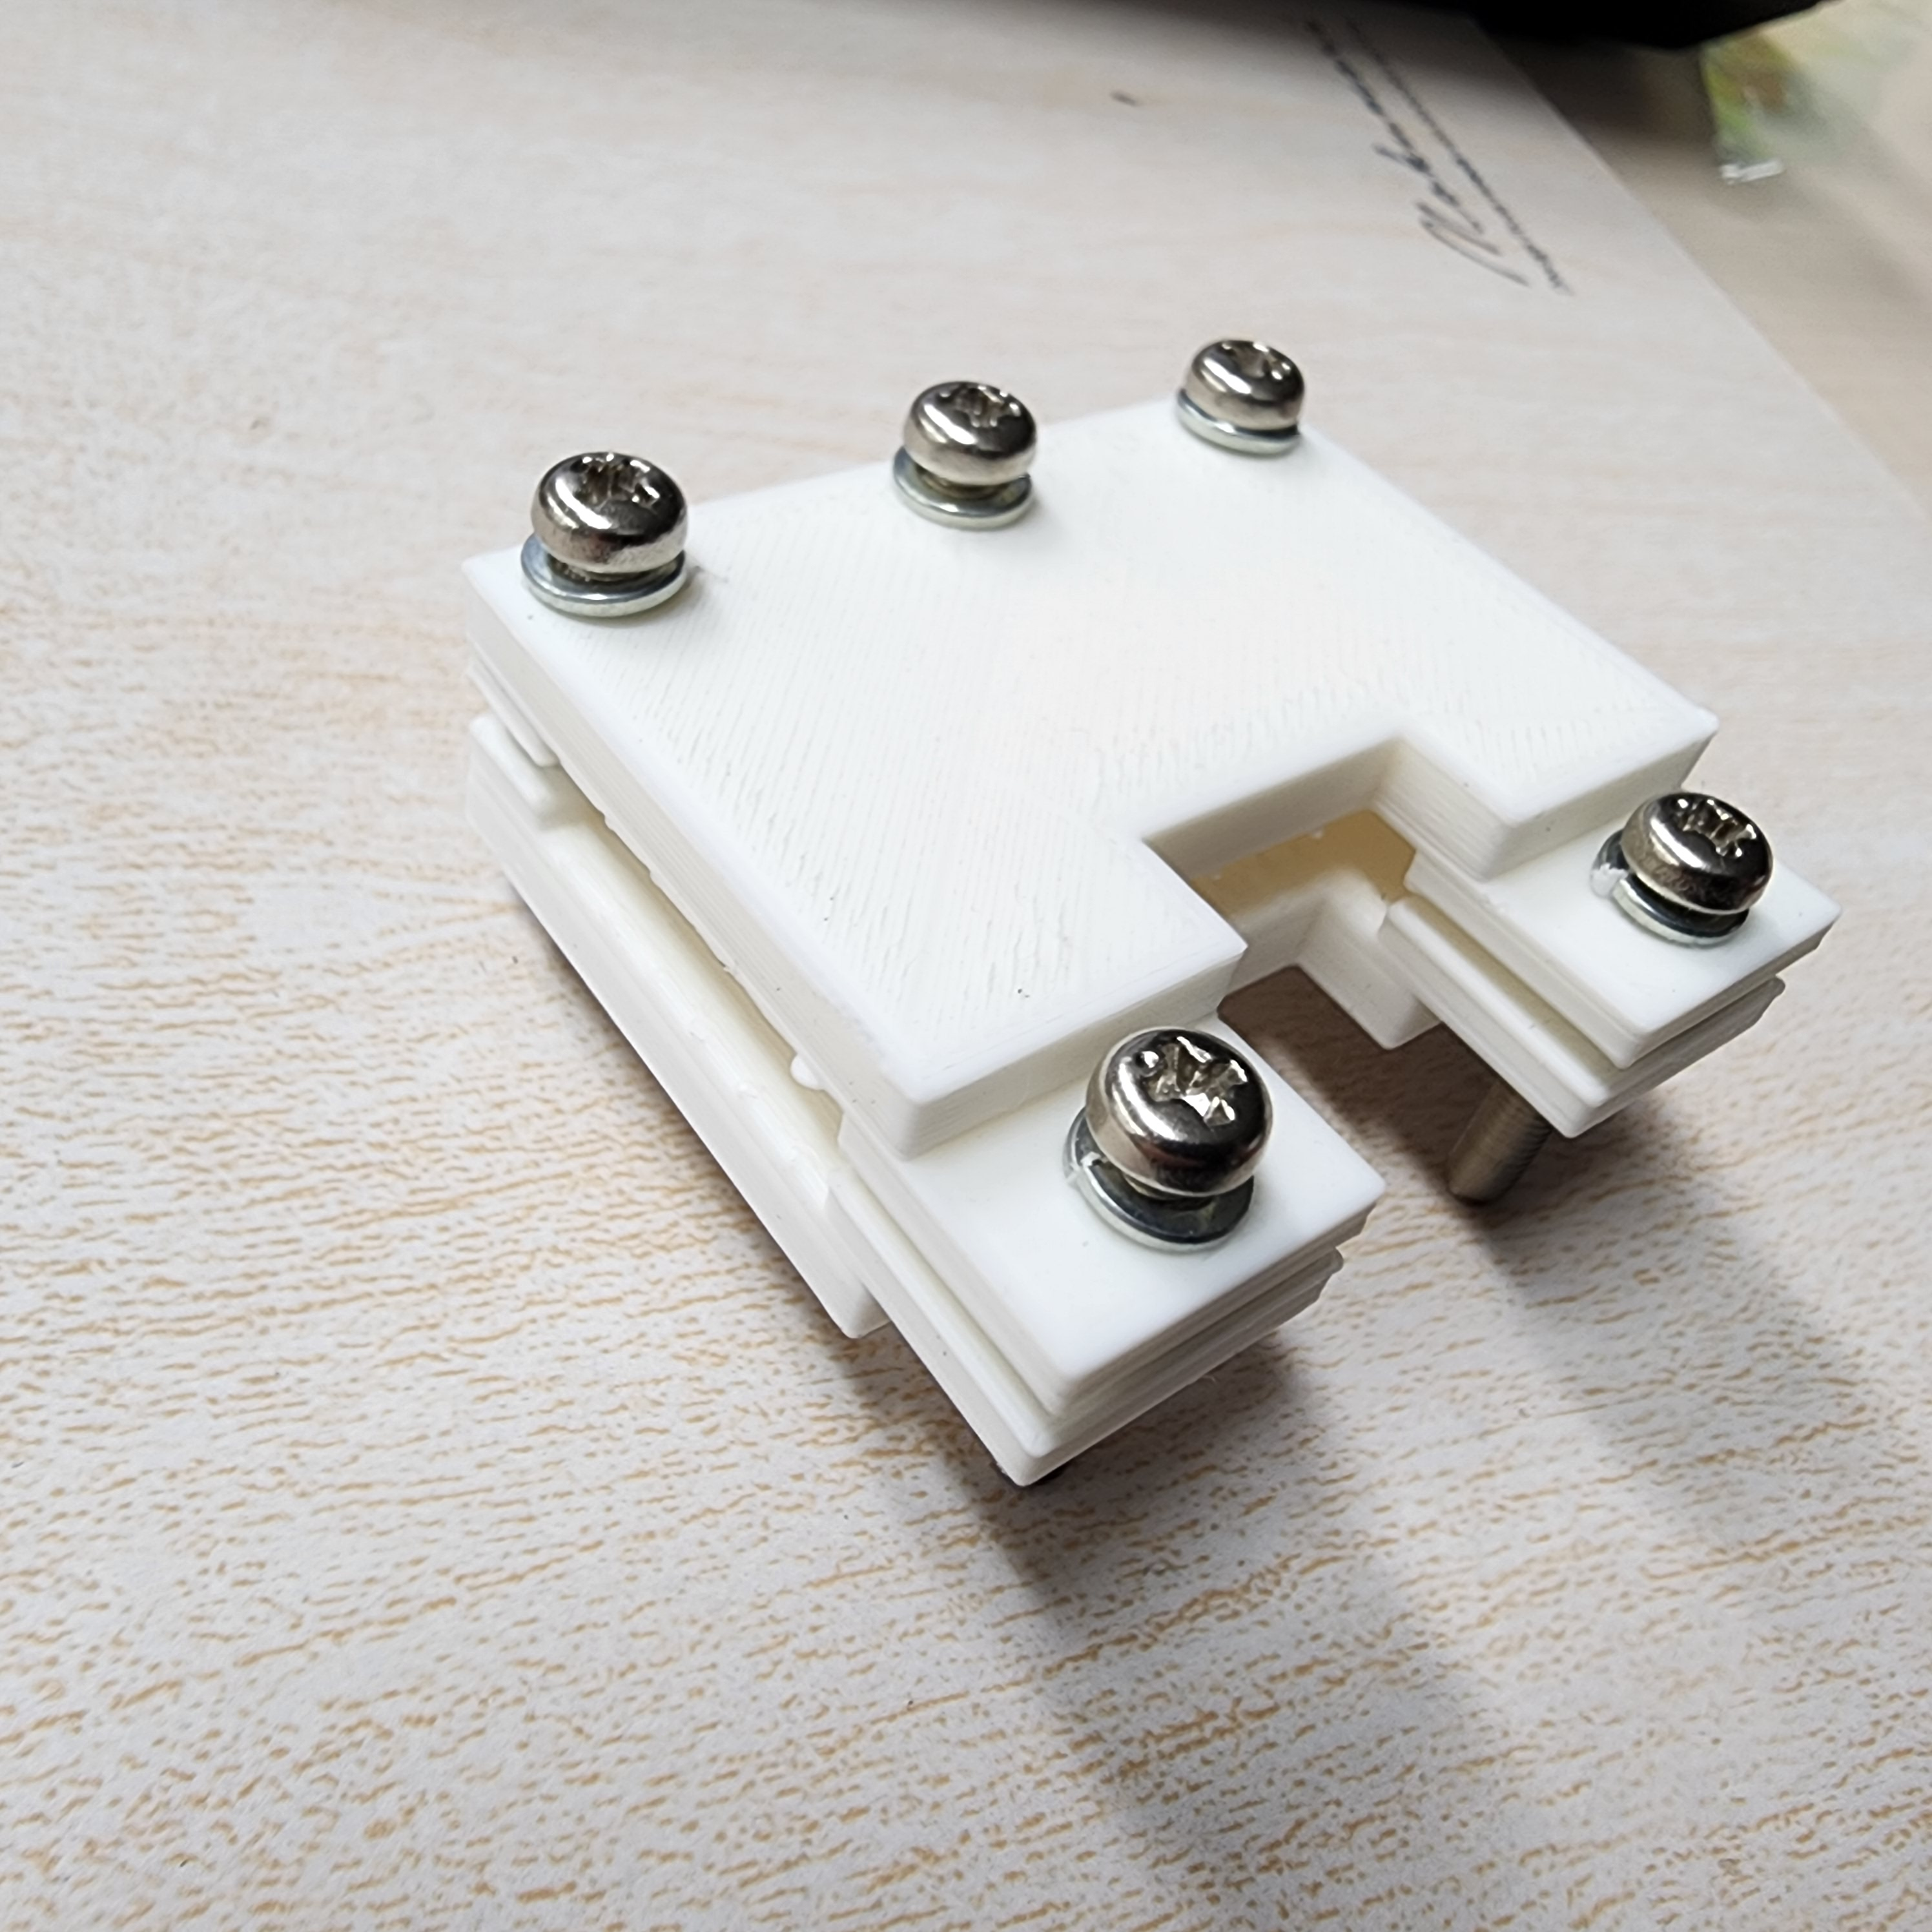
\includegraphics[width=0.6\textwidth]{A_thesis/figures/021.jpg}
\caption{3d design - fixture}
\end{figure}


After production, the device can achieve the most basic blade impact function. In simple terms, the relay is controlled to open and close through the development board, which can control the circuit where the solenoid is located. When the circuit is connected, the central part of the solenoid is pushed back under the action of electromagnetic force, and when the circuit is disconnected, the electromagnetic force returns to the default state, and the central part pushes forward to generate an impact force. The control logic inside the development board is to uniformly control the presence or absence of a digital signal, so that the user can feel a recoil force similar to the collision of swords in the virtual space.

\begin{figure}[h]
\centering
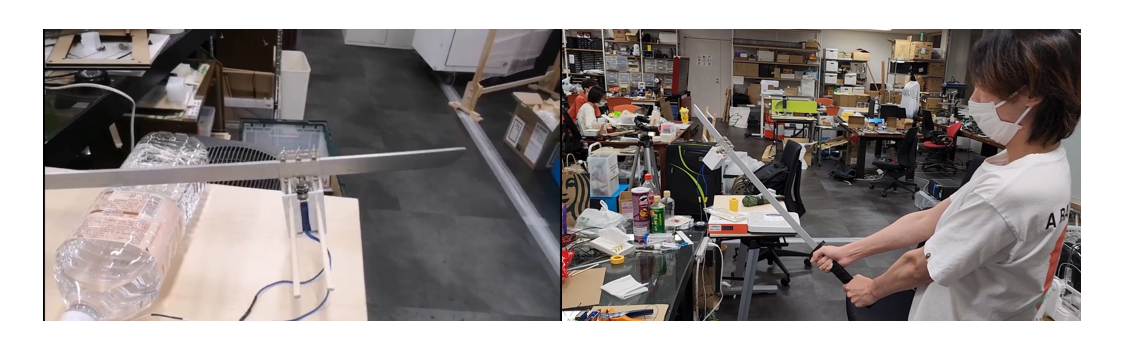
\includegraphics[width=0.95\textwidth]{A_thesis/figures/022.png}
\caption{Prototype and usage example}
\end{figure}


\subsection{Pilot Test 1}
After preliminary testing (n=5), the user's overall feedback was lower than expected.
There are several problems summarized as follows:
The overall weight is large, and the weight distribution is unreasonable. Firstly, the solenoid has a large self-weight. In addition, the hanging area is far from the user's hand grip area. The force arm is too long, leading to a higher design weight, and the weight cannot support the user to use the device freely. 
In addition to not achieving the expected effect in terms of kinematic haptic effects, users strongly suggest that visual information should be used to supplement the deficiencies. In other words, if only using this kinematic device, users are still confused about the application scenario of this device and the specific content of the information conveyed, and need visual guidance.

\section{Prototype Version 2 -zShape}
\subsection{Concept Design}
After the first round of production and testing, the second version of the prototype was modified based on the feedback received. The objective of the device remains consistent with the previous goal, aiming to develop a set that can simulate the user's handheld object movement status in a virtual environment, such as a weapon. The main modifications are as follows:

The device itself does not need to be consistent with reality in terms of length, for example, in the simulation of a samurai sword, the haptic device itself does not need to maintain the same length as the samurai sword. Therefore, the device will not use model knives as the main carrier, but will only use 3D printing to print the device body. The design should consider the user's grip method and pay attention to the tilt angle.
Considering the weight balance, not only the front end of the blade in the design needs a force generator, but also the back end of the device needs a force generator during the recoil process to ensure a certain degree of balance. It won't be too heavy on the front end of the device, making the user unable to control their behavior during use. For the selection of heavy objects, we chose the same solenoid as the front end for adjustment.
Since the existence of the blade is cancelled in the design, it is necessary to consider whether the inertia produced by the solenoid itself hitting the air can produce enough kinematic effects on the user, or use other objects to replace the blade as the impact point of the solenoid.

\begin{figure}[h]
\centering
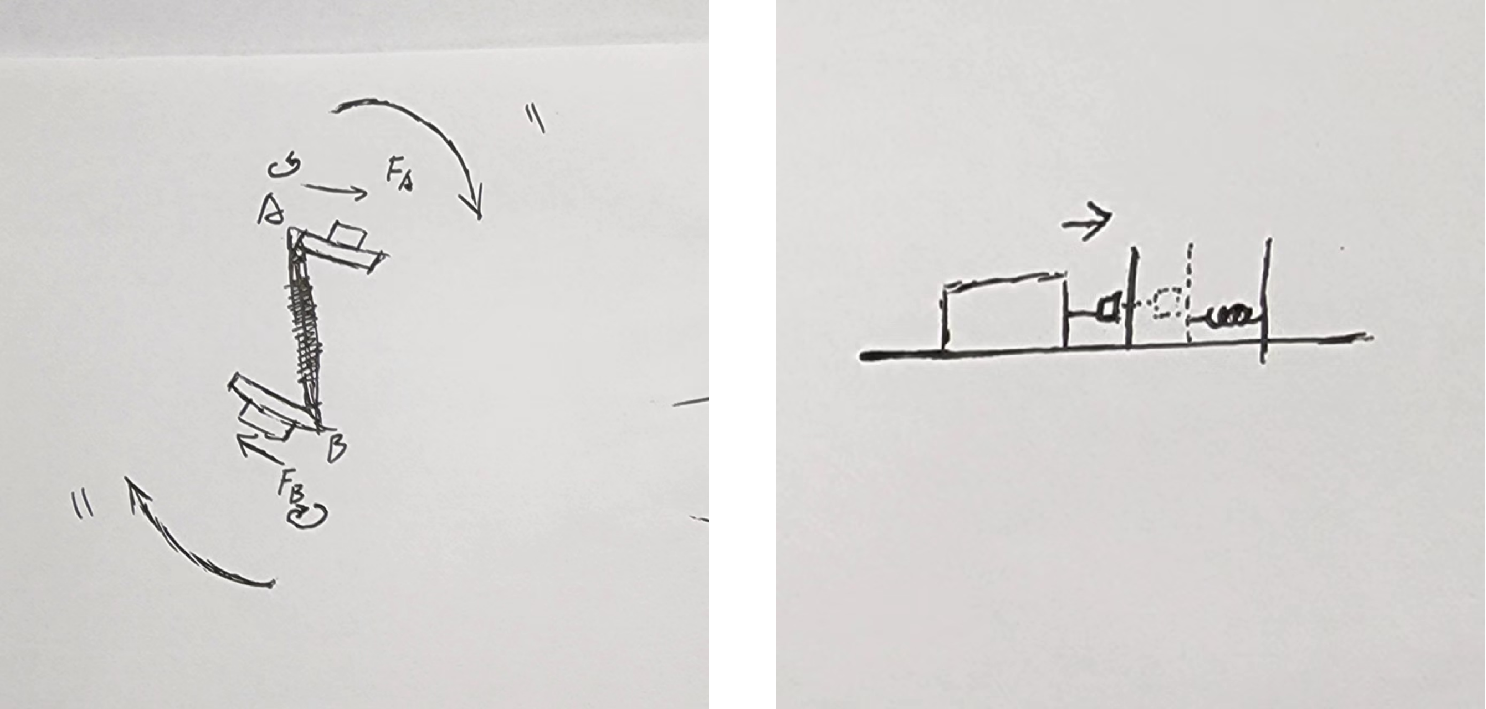
\includegraphics[width=0.6\textwidth]{A_thesis/figures/023.png}
\caption{Early design drafts 2}
\end{figure}

\subsection{Implement}
\subsubsection{Haptic Design}
In terms of heavy object configuration, we chose the same force generator as the previous prototype design, the solenoid, and used the same output model to ensure that the user has the same front and rear weight perception when using it. Also, according to the function design, the solenoid generates output in two opposite directions to simulate the impact force received and the recoil force after receiving the impact force.

\begin{figure}[h]
\centering
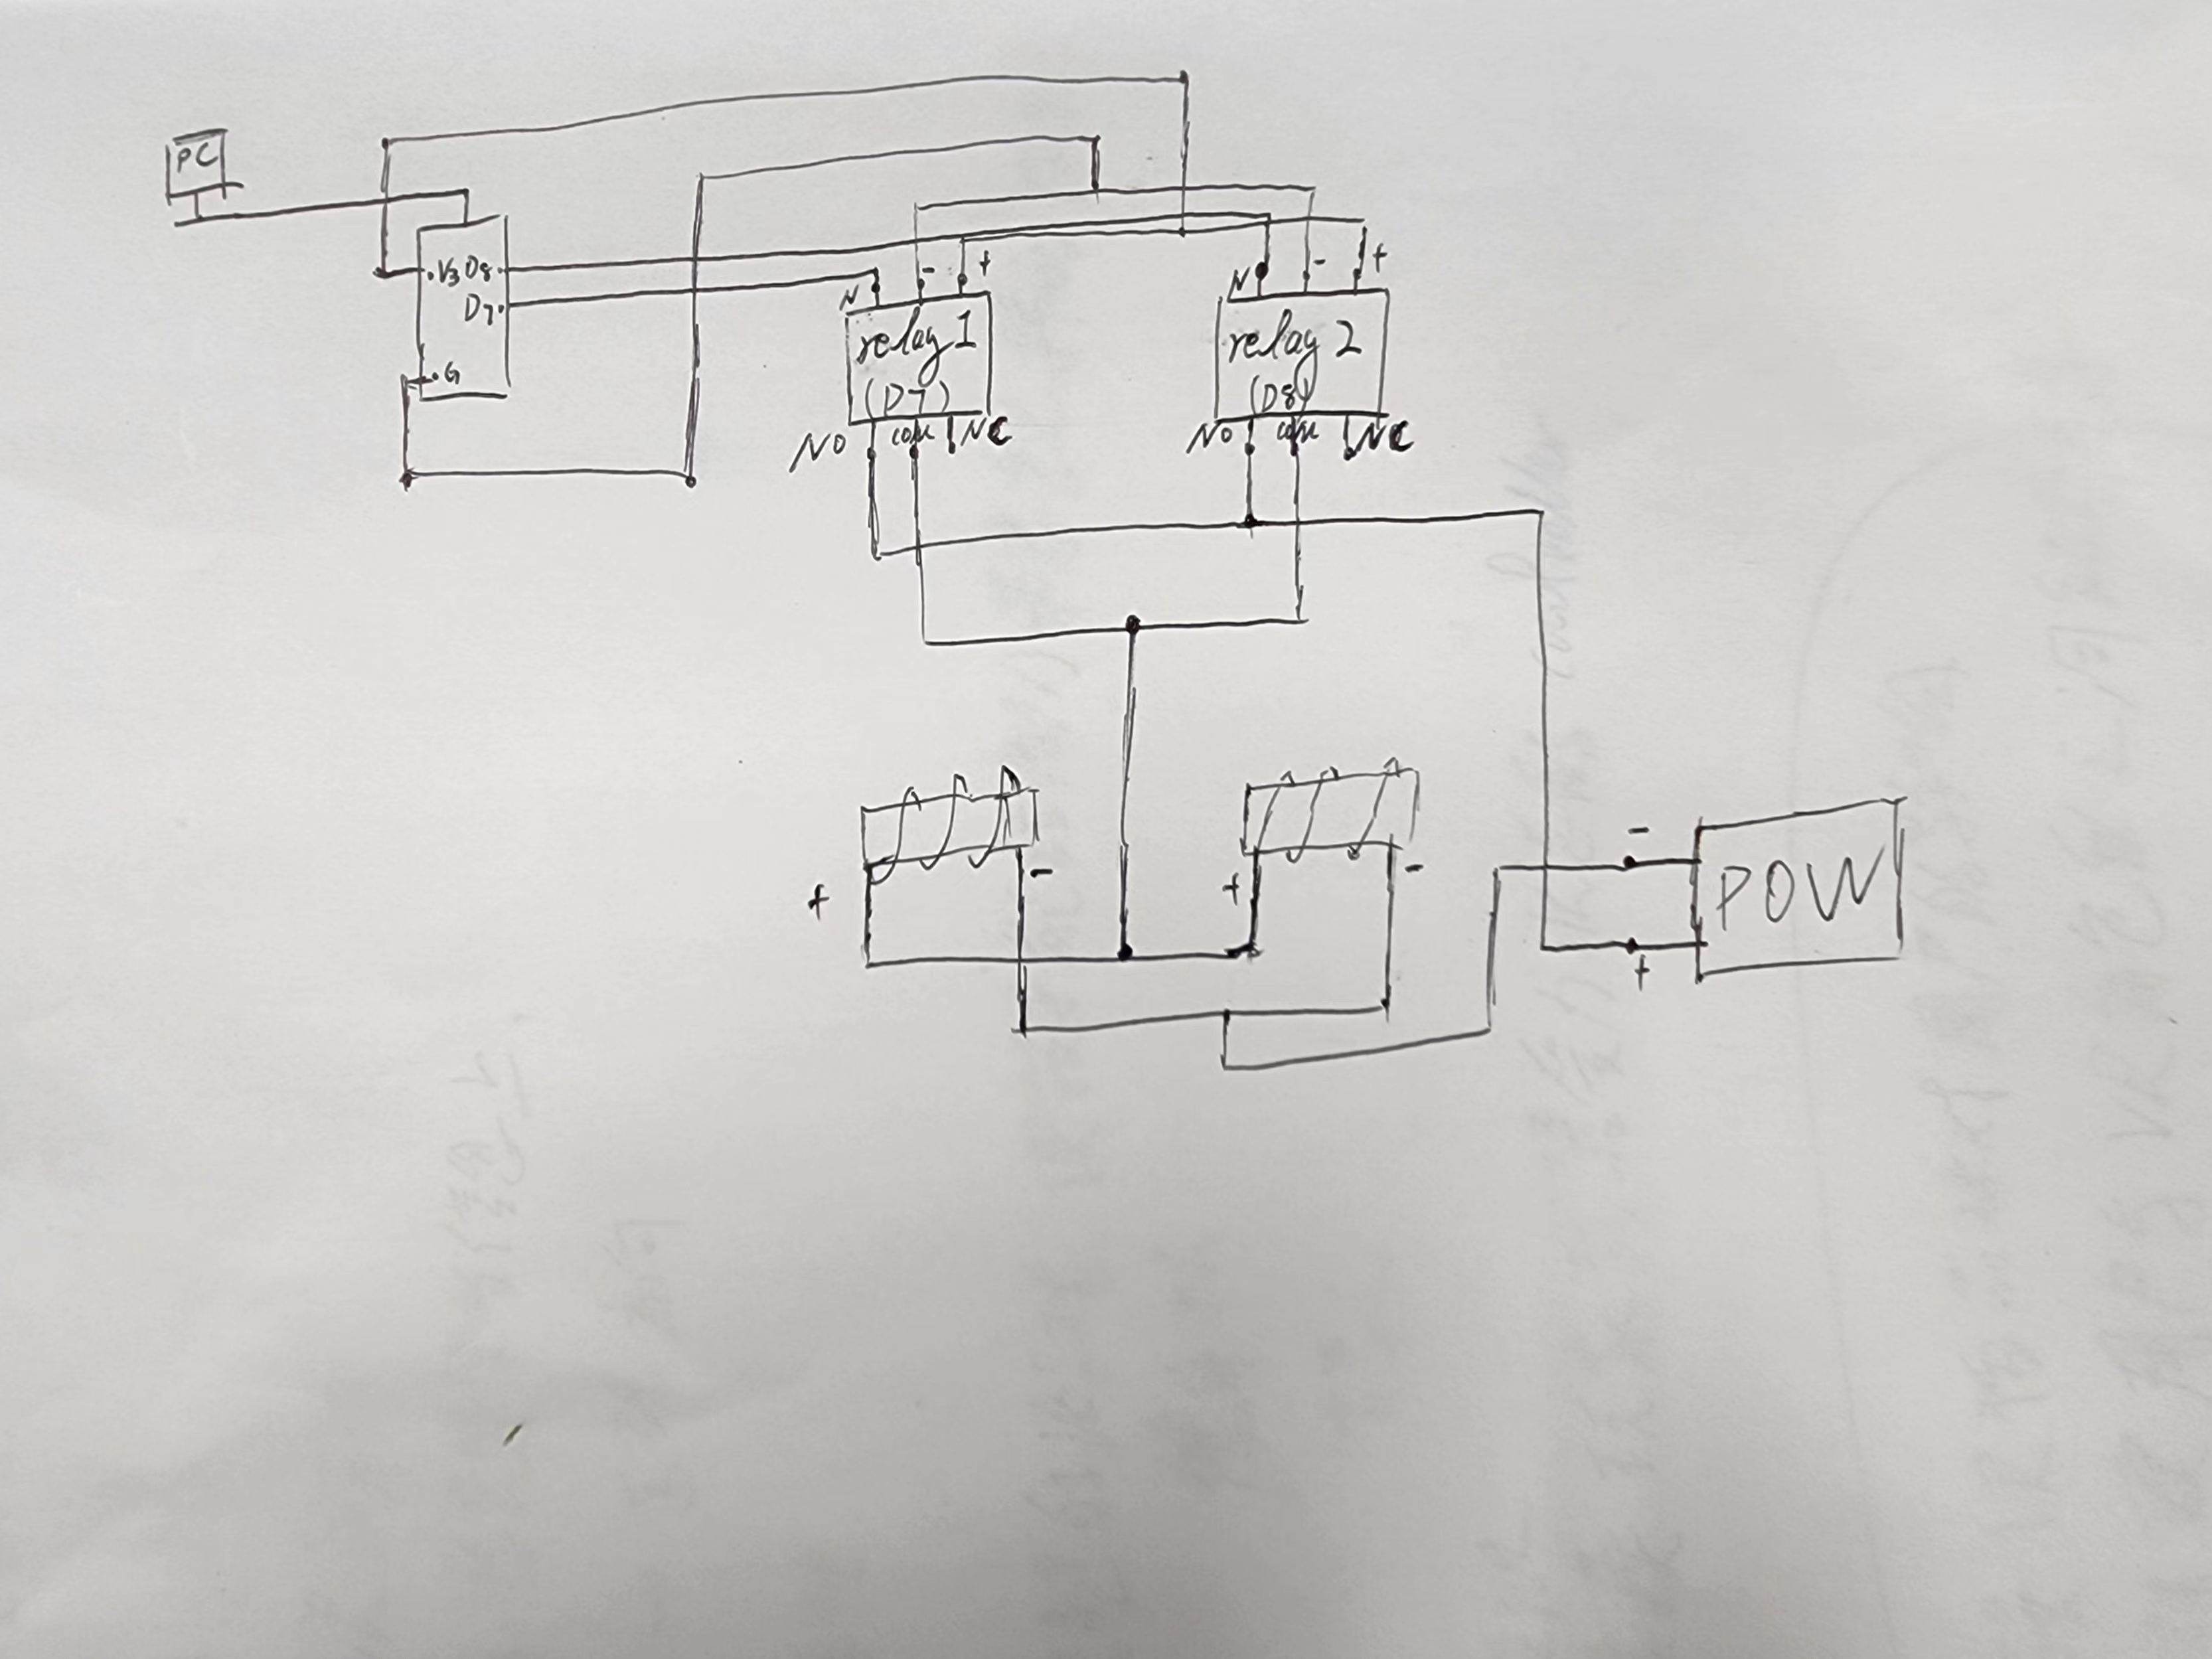
\includegraphics[width=0.6\textwidth]{A_thesis/figures/024.jpg}
\caption{Circuit diagram}
\end{figure}

\subsubsection{3D Design}
For the main body part, we chose a Z-shaped design. The inclined part in the middle is convenient for users to grip and has a certain angle to help the  device better adjust the output. The horizontal structure at the top and bottom is used to provide support for the solenoid base.
In the design of the impact part of the solenoid, a baffle is designed to accept the impact force generated by the solenoid. About the connection method between the baffle and the main body, two schemes have been tried, one is directly fixed to the bottom, and the other is to use rails and springs to make the baffle retractable. Specifically, the rail is dug out inside the base to ensure the movement path of the baffle, and a spring is added inside the rail to restore the baffle to its original position after being hit. However, after testing the actual effect, the kinematic effect of the rail plus the baffle is not as good as the effect of the baffle directly, so the baffle is still fixed on the base.

\begin{figure}[h]
\centering
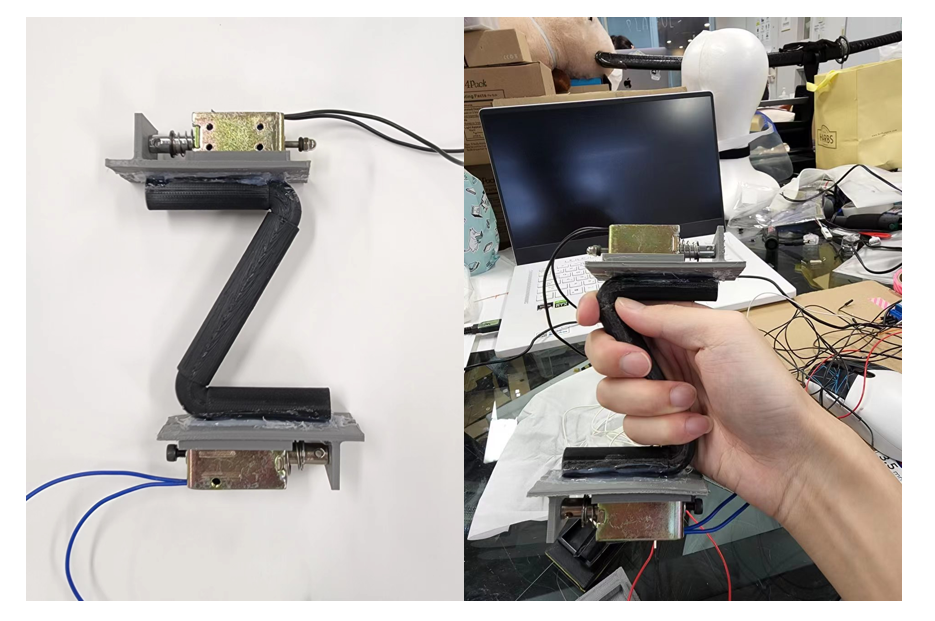
\includegraphics[width=0.6\textwidth]{A_thesis/figures/025.png}
\caption{Prototype display}
\end{figure}

\subsection{Pilot Test 2}
After production, a simple test (n=5) was also carried out. Compared with the previous time, the overall performance has significantly improved compared with the previous prototype, specifically in terms of smaller volume, lighter weight, and better balance. Because the shape is no longer a long strip type, so in the actual application process, the use method and simulation object are no longer limited to long sword-type weapons.
After the two-direction haptic output, the overall movement performance of the device has significantly improved, and people can feel the kinematic effects of advancing and retreating. At the same time, the output in the two directions has a larger adjustment space compared with the single output last time. That is to say, the solenoid can make fine adjustments in its own output mode, such as the solenoid at the rear end fires slightly later than the front end. It may will make the user feel the impact first, then feel the recoil, such a complete kinematic process of receiving force blocking.
However, in the testing process of this prototype, users still cannot understand the purpose of the device without the aid of visual information, and mentioned in the test that "The occurrence of action kinematic effects is very obvious. I know that a certain action has occurred when using the device, but I am still puzzled about what kind of action it is."

\subsection{Conclusion}
In addition to the problems of the device and system itself, there are still three core issues that have not been clearly answered in the entire design process. First, what kind of physical force is this haptic device focused on reproducing? Although the design goal is to hope that users can clearly feel their own action trajectory and direction when using this device, but in the application scenario of weapon swinging, which force is specifically reflected has not been clearly stated. 
Second, the limited application scenario, apart from the user's weapon fighting scene, are there any other potential application scenarios for this system? 
Third, in the design process, it is still a reproduction of the kinematic phenomena that exist in reality, rather than innovative interaction methods on how specific users interact with future technological content. It is necessary to consider some new interaction methods that do not currently exist or may appear in the future.

\section{Drone Research Project}
In addition to the exploration of haptic technology for motion, other research projects have been conducted. While their methods and contents are not the same as the main research topic of this project, they serve as an important reference for the development of future research.
The additional research content here is about using drones as the source of haptic output. Initially, the design was meant to use the 3DOF kinematic output of drones to produce effects on the human body, but it proved challenging to maintain a fixed distance between the drone and the user in the actual algorithm implementation. Ultimately, the drone was fixed on the user's head, and vestibular effects were used to create kinematic effects in multiple directions on the user's head to guide the user to navigate effectively.
In design, we connected the bottom of the open-source drone to a helmet, and the user wore the helmet to feel the physical cues provided by the drone to identify the direction of guidance. To disperse the weight of the drone, a wooden and cross structure was attached to the bottom of the drone and secured to the user's chest.
In the actual experiment (n=5), it was found that the method of guiding the user's direction through the drone could indeed guide the user to distinguish direction. In the second experiment, it was also found that the system could guide the user to the designated location without visual cues and relying solely on touch.

\begin{figure}[h]
\centering
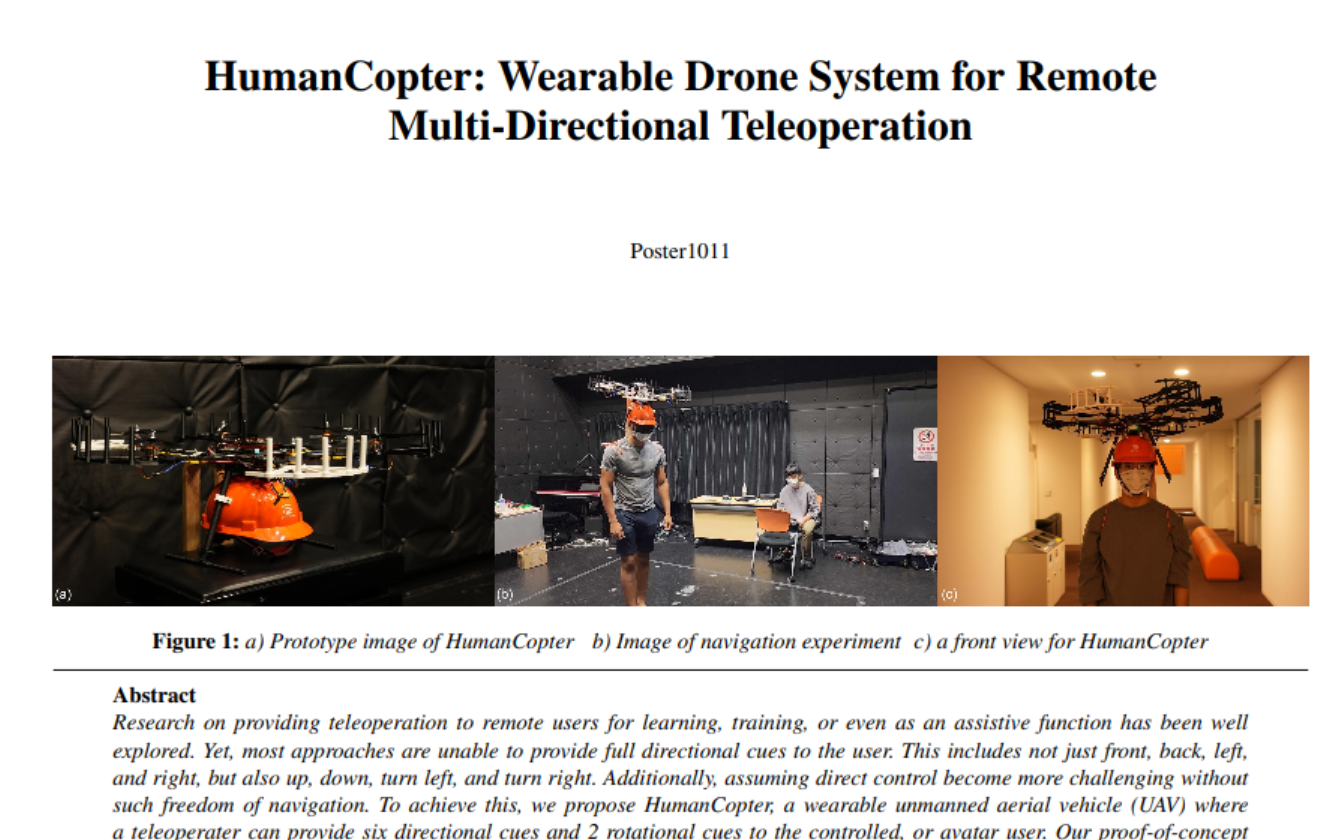
\includegraphics[width=0.75\textwidth]{A_thesis/figures/026.png}
\caption{Publication on drone research project}
\end{figure}


\section{Prototype Version 3 -1dof}
\subsection{Concept Design}
After the previous two attempts, the decision was made to tackle the core problem, i.e., to clarify the research direction. For clarity in the movement trajectory, it might be easier to start with smaller objects with a fixed movement path, such as a train or car that can only move forwards and backwards. Compared to the free actions of users, the human joints have a too high degree of freedom, making it hard to find the basic implementation targets and measurement methods. Therefore, the prototype design of this time started from the most basic movement action to reconsider and design the prototype.
Considering the changes in motion in multiple dimensions, after using the guide rail and tilt designs in previous research, it was found that the tilt design could not effectively represent the accurate distance and feeling of movement in long-term movement. Hence, in the early design of this time, two design schemes were attempted:

Design 1:
Installing three wheels on a handle-like component, each wheel representing movement in one dimension of XYZ, hoping that such a setting could convey the motion information in XYZ dimensions to the user.
\begin{figure}[h]
\centering
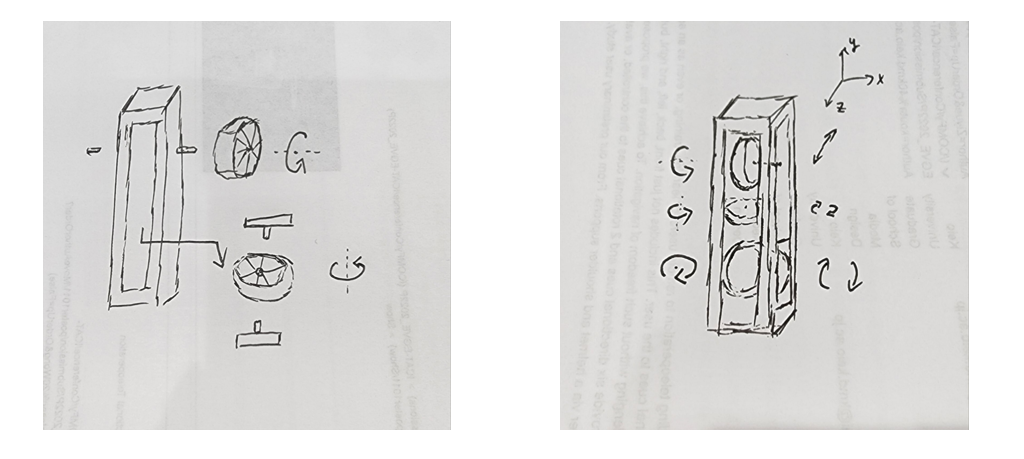
\includegraphics[width=0.8\textwidth]{A_thesis/figures/027.png}
\caption{Design drafts for design 1}
\end{figure}

Design 2:
Placing a vibrator in each direction of the device, using the vibration information of the vibrator to represent different motion states of the object (in the figure, the yellow cylinder represents a vibrator, and the blue represents the support structure).

\begin{figure}[h]
\centering
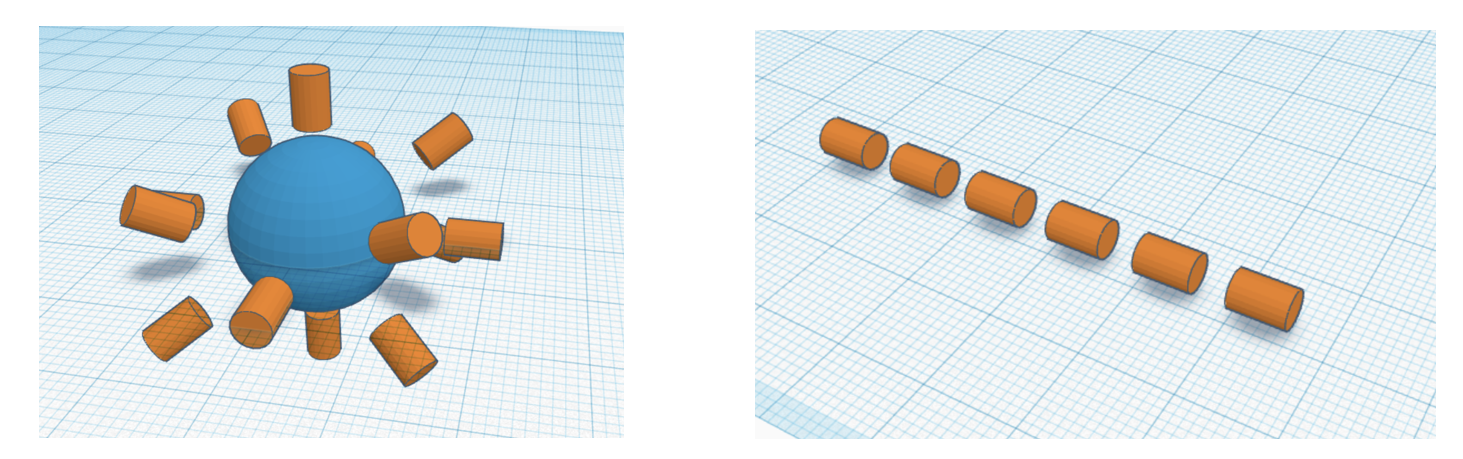
\includegraphics[width=0.8\textwidth]{A_thesis/figures/028.png}
\caption{Design drafts for design 2}
\end{figure}


After subsequent discussions, the first scheme was chosen, that is, using the forward and backward rotation of the wheel to represent the forward or backward movement of the object in virtual space.And at the beginning of the attempts, will focus on exploring the dimension of 1 degree of freedom (1dof). This will build upon our previous attempts, gradually advancing our design and development efforts towards more complex 3 degrees of freedom (3dof) devices.

\subsection{Implement}
\subsubsection{Haptic Design}
In terms of implementation, an Arduino 360 servo was used as the final kinematic performance device. A 3D printed shell was installed on the top of the servo, and it was hoped that users could feel the same motion situation in the virtual space by feeling the rotation of the external touch lid.
Furthermore, the push-pull structure of the crank was tried, and a shell was placed on the user's hand. The internal flat structure combination was used to express the advance and retreat of the object by means of thrust and pull. However, the kinematic performance was significantly weaker than the wheel structure.
In terms of system control, Unity and Arduino were used for serial communication, using Unity to transfer parameters to adjust the digital output signal of Arduino to control the servo. Users can control the rotation of the server by controlling the direction key.

\begin{figure}[h]
\centering
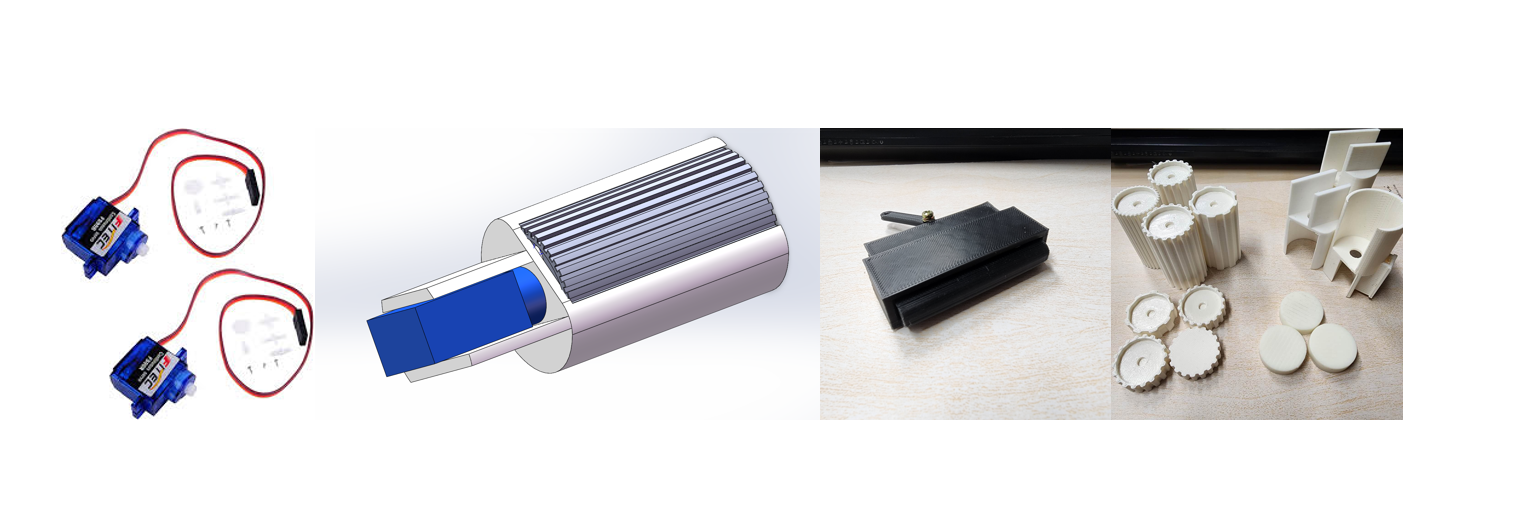
\includegraphics[width=0.9\textwidth]{A_thesis/figures/029.png}
\caption{Research process (3650 servo, 3d design, crank design, 3d printing)}
\end{figure}

\subsubsection{3D Print}
Using the 3D printed structure, the part that the user touches and the rotating part of the servo were separated. Depending on the different parts of contact, the kinematic effects produced are also different. For example, in the internal tests, the moving servo parts responsible for the forward and backward movement direction have weaker haptic effects than those interacting with the user's fingertips because they mainly contact the inside of the hand (including the inside of the fingers and the palm). The texture of the contacted object's surface also has different effects on the kinematic expression. For instance, a surface with a concave and convex texture can produce stronger haptics than a smooth surface, but too many bumps may cause pain during use. Therefore, after tests, a moderate concave and convex surface was chosen to ensure effective haptics without causing pain to the user during use.
In addition, according to the tests, the kinematic effect provided by the rotating movement varies depending on the relationship between the rotating contact area and the position of the palm. The kinematic performance when the rotation axis is parallel to the palm surface is significantly weaker than when they are cross-vertical. Based on the above tests and adjustments, the final choice was to increase the contact area to improve the user's experience.

\subsubsection{System Design}
In system construction, Unity was not only used as the main control interaction interface but also for building a visual prompt application scenario for users. A simulated driving system was set up in Unity. In such an application scenario, users can control the movement of the car in the scene to synchronously rotate the servo in the handheld device.

\begin{figure}[h]
\centering
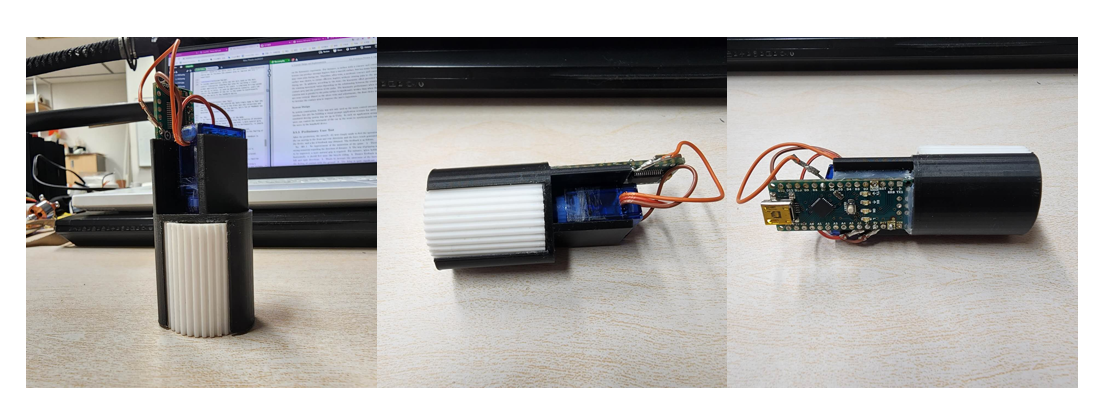
\includegraphics[width=0.9\textwidth]{A_thesis/figures/030.png}
\caption{Three views of the prototype}
\end{figure}


\subsection{Preliminary User Test}
After the production, the users(N =6) were simply made to feel the operation of the car moving in the front and rear directions and the force touch generated by the device, and a lot of feedback was obtained. The feedback is as follows.

No. 001:    1. No improvement of the immersion of the game.
2. There's a strong sensation regarding the direction of distance.
3. The way of gripping needs to be improved, a more natural grip is required. For instance, when holding it horizontally, it should feel more like bicycle riding.
4. Desires feedback in the left and right directions.
5. Wants to increase the awareness of the tires and the feeling of contact with the ground.
6. The delay is quite significant, more immediate feedback is desired.

No. 002:    1. There's a distinct feeling of moving forward.
2. The tactile feeling of moving forward and backward is inconsistent.
3. The contact area with the palm needs to be well planned.
4. Desires a diagonal forward direction.
5. There might be a greater enhancement for visually impaired individuals.
6. When used in a video or racing environment, providing a corresponding sense of speed would be more immersive and increase the distance between the user and the racer.

No. 003:    1. Desires force feedback in the left and right directions.
2. Bugs and delay greatly affect the overall immersive physical experience.
3. The choice of Vection in the forward and backward direction has an impact on the user.
4. The method of grip requires moderate pressure, to avoid being too hard to turn, or too light to feel.
5. Continue fixing bugs.

No. 004:    1. Desires the inertial feeling of stopping when finally parking.
2. Wants the feeling of acceleration pushback.
3. Considering how to integrate with the controller.

No. 005:    1. There's no sense of unity between the controller and the system.
2. Visual impact?
3. The feeling in the two directions is inconsistent.
4. The rotation towards one's own body direction is more intense.

No. 006:    1. The sensation of moving direction is very strong.
2. Holding with one hand and operating with the other creates a serious feeling of disconnection.
3. Wants feedback of the dull feeling when stopping and the vibration of movement.
4. Integration with the joystick? Embedding?

\section{Prototype Version 4 -2dof}
\subsection{Concept Design}
After the previous testing, the system first and foremost presented a very obvious kinematic effect, and the user's physical sensation also successfully approached the research goal, i.e., feeling the moving state of the moving object, including the moving direction and rotation angle. However, there were still some missing details, such as the relationship of velocity vectors. Moreover, due to the application scenario, most users demanded not only the kinematic feedback of the 1dof forward and backward, but also strongly required at least the corresponding kinematic feedback in the left and right directions. Additionally, some aspects of the system needed to be optimized, such as reducing communication latency, decreasing the duration of single rotation, increasing the update detection frequency, and considering other possible application scenarios outside of the device's kinematic effects, such as whether it can enhance the user's connection with the virtual vehicle.

\subsection{Implement}
According to the requirements from the previous user test, the system update mainly provided rotation in the left and right directions. A 360-degree server in the left and right directions was set up in the center of the user's palm, parallel to the user's palm. Due to the natural curve of the human hand during use, the edges of the cover were beveled to avoid pain during use.
Additionally, the system settings changed the third-person perspective to a first-person perspective, better simulating the user's real experience in a driving environment. 

The system is not only in positive correlation with the direction and angle of moving objects in virtual space,  the rotation speed of the device would also change in real time according to the speed of the virtual object. The adjustments in the system also included increasing the refresh rate of the serial communication, raising it from the original refresh rate to the current one, and reducing the duration of a single rotation. This effectively avoided communication backlog in the serial port, where the signal processing time of the first input is too long, leading to the inability of the subsequent input signal to be processed in time.

\subsection{Functional Explanation}

This sections will delineate the functionality and operational methodology of the prototype developed in this research. 

The device consists of two servo motors, referred to as Servo1 and Servo2. 
\begin{figure}[h]
\centering
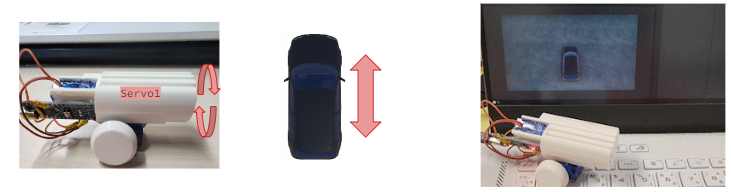
\includegraphics[width=0.9\textwidth]{A_thesis/figures/033.png}
\caption{Illustration of servo1}
\end{figure}
Servo1 is horizontally positioned within the central chamber and interconnected with a rotating wheel. The surface of this wheel makes contact with the user's inner finger. When there is a displacement in the vehicular movement within the virtual environment, either forward or backward, Servo1 initiates a rotational movement. This allows the user to perceive the locomotive state of the virtual vehicle through the friction between their finger and the wheel. Specifically, forward motion in the virtual vehicle prompts a clockwise rotation of the wheel, while a backward motion triggers a counter-clockwise rotation.
\begin{figure}[h]
\centering
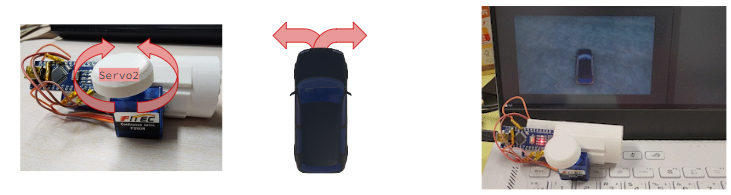
\includegraphics[width=0.9\textwidth]{A_thesis/figures/034.png}
\caption{Illustration of servo2}
\end{figure}
Servo2, placed externally on the device, is linked with a turning wheel, the surface of which interacts with the user's palm center. This arrangement facilitates the conveyance of rotational information concerning the vehicle within the virtual environment to the user via the wheel's movement. When the virtual vehicle pivots either to the left or right, Servo2 responds by rotating in the respective direction. Thus, a leftward rotation of the virtual vehicle results in a leftward wheel movement, while a rightward vehicle rotation induces a rightward wheel movement.

\begin{figure}[h]
\centering
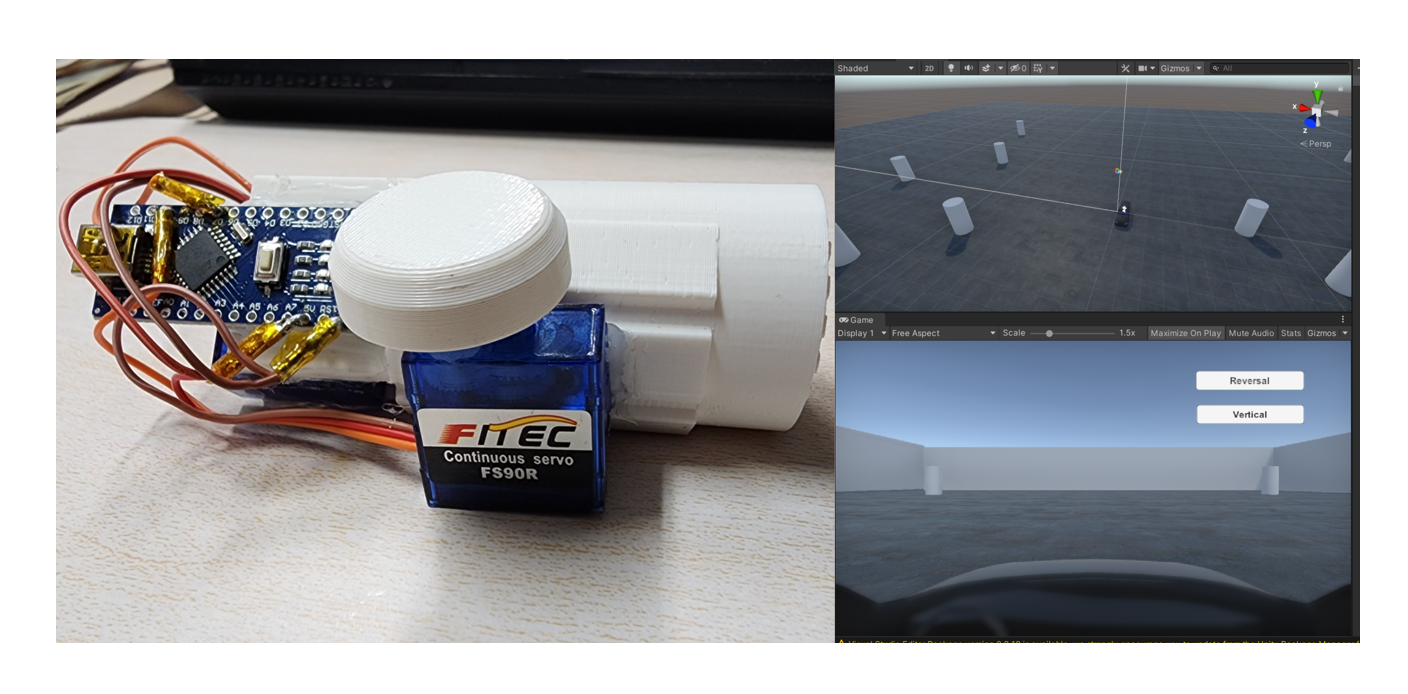
\includegraphics[width=0.9\textwidth]{A_thesis/figures/031.png}
\caption{Final prototype and virtual environment demonstration}
\end{figure}
Concerning the user interaction interface, as depicted in Figure 3.16, a simple virtual vehicular movement scenario has been created using Unity3D. The setting comprises walls, minor mazes, and cylindrical obstructions at randomized locations, simulating a conventional road scenario to approximate the real-world user environment as closely as possible. Users observe from a first-person perspective and can manipulate the vehicle's movement - forward, backward, left, and right - using the directional keys on the keyboard. In tandem with accepting control signals, Unity3D also transmits them to the MotionPerformer via serial communication.


\textbf{For the coding of unity and arduino, please refer to the appendix 'A' and 'B'.}